\subsection{ILASP}

ILASP enables learning programs containing normal rules, choice rules and both hard and weak constraints, these are the rules that compose ASP econdings and here this tool will be used for the maze problem. Weak constraints won't be covered, the goal here is to try to learn some rules that will form an encoding of that problem.

\subsubsection{Learning normal rules - learning how to walk}

The first task is learning to walk on the maze, considering adjacent cells and the obstacles (walls and co.). This task have been split for complexity reasons, as a result first it will be learned how to move on near cells and then obstacles will be considered, in 2 different ILASP scripts. Here some normal rules will be learned, in the next sections other kind of rules will be covered (regarding the same problem).

\subsubsection{Learning to walk on adjacent cells}

this is the ilasp code written for the pourpose, with some bit of background knowledge, definition of search space with language bias and some examples with all different "cases".  Finding those examples has been pretty difficult because they must be meaningful and as such must capture all the different contexts.

\newpage
\begin{lstlisting}[language=Prolog]
%%%%%%%%%%%%%%%%%%%%%%%%learn how to move on near cells
row(1..5).
col(1..5).

cell(X,Y) :- row(X), col(Y).

succ(0,1).
succ(X, X+1) :- cell(X,_).

%%%%%%%%%%%%%%%%%%%%%%%%%%%%%SEARCH_SPACE + EXAMPLES
#pos(p1, {next((4,2), (4,1)), next((4,2), (4,3)), next((4,2), (3,2)), next((4,2), (5,2))}, {}).
#pos(p2, {next((2,3), (2,2)), next((2,3), (1,3)), next((2,3), (2,4)), next((2,3), (3,3))}, {}).

%no out of range or jump
#neg(a, {next((1,0), (1,1))}, {}).
#neg(b, {next((1,1), (0,1))}, {}).
#neg(c, {next((0,1), (1,1))}, {}).
#neg(d, {next((1,1), (1,0))}, {}).
#neg(e, {next((5,5), (6,5))}, {}).
#neg(f, {next((5,5), (5,6))}, {}).
#neg(g, {next((6,5), (5,5))}, {}).
#neg(h, {next((5,6), (5,5))}, {}).
%no diagonal move
#neg(i, {next((2,4), (1,3))}, {}).
#neg(l, {next((2,4), (1,5))}, {}).
#neg(m, {next((2,4), (3,5))}, {}).
#neg(n, {next((2,4), (3,3))}, {}).
%no move same cell
#neg(o, {next((2,4), (2,4))}, {}).

#modeb(2, cell(var(r), var(c)), (positive, anti_reflexive)).
#modeb(1, succ(var(c), var(c)), (positive, anti_reflexive)).
#modeb(1, succ(var(r), var(r)), (positive, anti_reflexive)).
#modeh(next((var(r), var(c)), (var(r), var(c)))).

#maxv(3).
\end{lstlisting}
At \ref{fig:asd} the output of the script, with the learned rules, ILASP actually learned that "next" predicate is true for adjacent cells, based on that the movement on the grid will be possible.

\begin{figure}
	\centering
	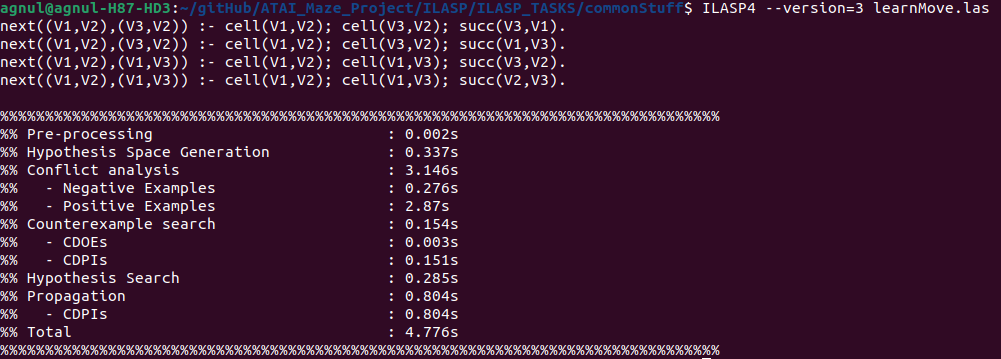
\includegraphics[scale=0.5]{img/learnMoveAdj.png}
	\caption{Learned rules - adjacent move}\label{fig:asd}
\end{figure}

\newpage
\subsubsection{Learning to walk on cells without obstacles}
The next step is to consider obstacles on the grid, as discussed on the "background knowledge" in (ref). Here the goal is to find a new normal rule that represent the concet of a "valid move", in a cell without obstacles.

\newpage

\begin{lstlisting}[language=Prolog]
%%%%%%%%%%%%%%%%%%%%%%%%%%%%%%learn how to move on cells without obstacles
row(1..5).
col(1..5).

obstacle(1,2).
obstacle(2,2).
obstacle(3,2).
obstacle(3,3).
obstacle(4,3).
obstacle(4,4).
obstacle(3,4).
obstacle(2,4).
obstacle(1,4).
obstacle(1,5).
obstacle(5,1).

start(1,1).
goal(5,5).

%%%%%%%%%%%%%%

cell(X,Y) :- row(X), col(Y).

succ(0,1).
succ(X, X+1) :- cell(X,_).

%PATHS ADJACENTS (learned from previous ilasp task)
next((V1,V2),(V3,V2)) :- cell(V1,V2), cell(V3,V2), succ(V3,V1).
next((V1,V2),(V3,V2)) :- cell(V1,V2), cell(V3,V2), succ(V1,V3).
next((V1,V2),(V1,V3)) :- cell(V1,V2), cell(V1,V3), succ(V3,V2).
next((V1,V2),(V1,V3)) :- cell(V1,V2), cell(V1,V3), succ(V2,V3).


%%%%%%%%%%%%%%%%%%%%%%%%%%%%%SEARCH_SPACE + EXAMPLES

#pos(po, {nextLegit((1,1),(2,1))}, {}).
#pos(po2, {nextLegit((4,1),(4,2))}, {}).

%no movement on obstacles
#neg(a, {nextLegit((1,1),(1,2))}, {}).
#neg(av, {nextLegit((3,2),(4,2))}, {}).
#neg(af, {nextLegit((1,2),(1,1))}, {}).
#neg(b, {nextLegit((4,1),(5,1))}, {}).
#neg(g, {nextLegit((3,3),(2,3))}, {}).

#modeb(1, next((var(r), var(c)), (var(r), var(c)))).
#modeb(2, obstacle(var(r), var(c))).
#modeh(1, nextLegit((var(r), var(c)), (var(r), var(c)))).

#maxv(3).
\end{lstlisting}
At \ref{fig:asd2} the output of the script, with the learned rules, ILASP actually learned this new "nextLegit" predicate that represent the concept of a valid move: a move from (or to) cells without obstacles.

\begin{figure}
	\centering
	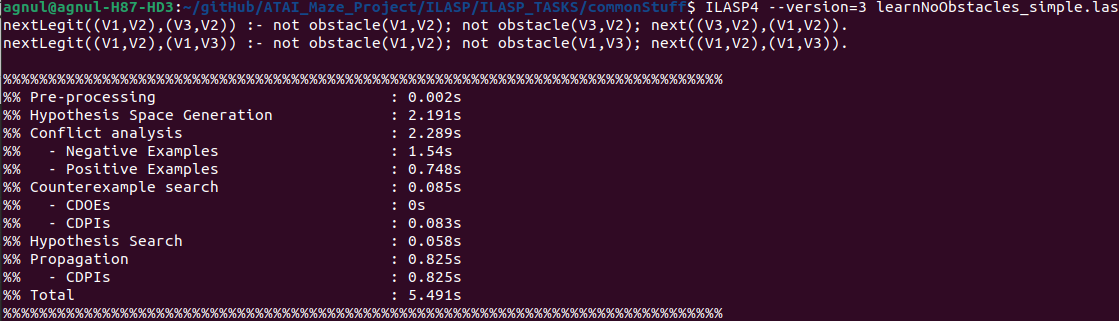
\includegraphics[scale=0.45]{img/learn_noObstacles.png}
	\caption{Learned rules - avoid obstacles}\label{fig:asd2}
\end{figure}

\newpage

\subsubsection{using this rules to define an ASP model}
having this rules in hand now is possible to define a model that solves our problem. Learned rules are reported exactly as they were on the ILASP scripts output. Some pieces are missing: some other rules need to be defined but they are quite intiuitive at this point. The code will be reported with the same grid discussed in ...
 
\begin{lstlisting}[language=Prolog]
	%MODEL THAT SOLVES PROBLEM OF PATHFINDING IN THE GRID
	row(1..5).
	col(1..5).
	
	obstacle(1,2).
	obstacle(2,2).
	obstacle(3,2).
	obstacle(3,3).
	obstacle(4,3).
	obstacle(4,4).
	obstacle(3,4).
	obstacle(2,4).
	obstacle(1,4).
	obstacle(1,5).
	obstacle(5,1).
	
	start(1,1).
	goal(5,5).
	
	%for each position define cell pred.
	cell(X,Y) :- row(X), col(Y).
	
	%FIND A PATH FROM START
	move(0,0,X,Y) :- start(X,Y).
	%for each "move" find another linked to it that is a legit move!
	1{move(X,Y,X1,Y1): nextLegit((X,Y), (X1,Y1))}1:- move(_,_, X,Y), not goal(X,Y).
	
	succ(0,1).
	succ(X, X+1) :- cell(X,_).
	
	%LEARNED BY ILASP, move on adj cells.
	next((V1,V2),(V3,V2)) :- cell(V1,V2), cell(V3,V2), succ(V3,V1).
	next((V1,V2),(V3,V2)) :- cell(V1,V2), cell(V3,V2), succ(V1,V3).
	next((V1,V2),(V1,V3)) :- cell(V1,V2), cell(V1,V3), succ(V3,V2).
	next((V1,V2),(V1,V3)) :- cell(V1,V2), cell(V1,V3), succ(V2,V3).
	
	%LEARNED BY ILASP, move on adj cells. without obstacles
	nextLegit((V1,V2),(V3,V2)) :- not obstacle(V1,V2); not obstacle(V3,V2); next((V3,V2),(V1,V2)).
	nextLegit((V1,V2),(V1,V3)) :- not obstacle(V1,V2); not obstacle(V1,V3); next((V1,V2),(V1,V3)).
	
	%ON GOAL POSITION STOP
	:- goal(X,Y), not move(_,_, X,Y).
	
	#show move/4.
\end{lstlisting}

at \ref{fig:asd3} the execution of "clingo" command on this model is shown: the path is represented by the chaning "move" predicate.

\subsubsection{performance test}
The work done with ilasp shows clearly this fact: the time complexity doesn't scale well with respect to the search space dimension. In fact, when trying to learn the "move to adjacent cells AND without obstacles" (the 2 tasks on the same scrit) compexity costs exploded "simply" for the insertion of the predicate "obstacle". (for a total of ... predicates in the search space). it is quite evident that a sort of exponential trend is in place and here I will like to do a specific test to demonstrate this.




\newpage
\begin{figure}
	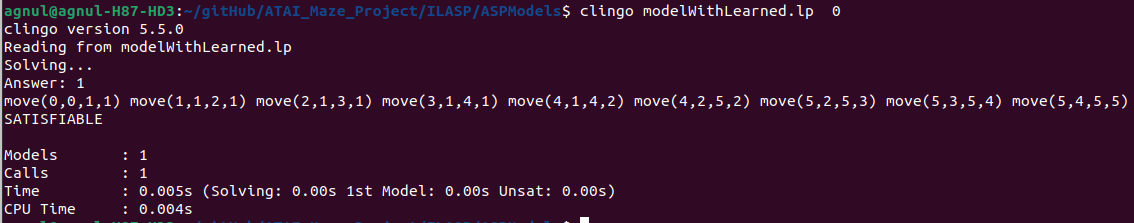
\includegraphics[scale=0.45]{img/outputModel.png}
	\caption{Path found on the grid}\label{fig:asd3}
\end{figure}


\newpage